%!TEX encoding = UTF-8 Unicode
% $Id: 5-returning_functions.tex 17 2014-03-09 13:05:41Z binghe $

\chapter{函数作为返回值}
\label{chap:returning_functions}
\index{functions 函数!as return values}

上一章展示了~Lisp~``把函数作为参数传递''的能力,它开阔了我们进行抽象的思路。我们对函数能做的事情越多,
就越能充分利用这些思想方法。如果能定义一种函数,让它产生并返回新的函数,
那就可以成倍放大那些以函数作为参数的\utility{}的威力。

这一章要介绍的\utility{}就被用来操作函数。要是把它们中的多数写成宏,让这些宏来操纵表达式
会显得更自然一些,
至少在~Common Lisp 里是这样的。在第~\ref{chap:macro_returning_functions}
章会把一层宏加到这些操作符之上。
不管怎样,就算最终这些函数仅仅被宏调用,``了解哪些工作能由函数来完成'' 这一点也至关重要。

\section{Common Lisp 的演化}
\label{sec:common_lisp_evolves}

Common Lisp 最初提供了几组互补的函数。\texttt{remove-if} 和~\texttt{remove-if-not}
就是这样的一对。倘若~\texttt{pred} 是一个参数的谓词,那么
\begin{lstlisting}
(remove-if-not #'pred lst)
\end{lstlisting}
就和下面语句等价
\begin{lstlisting}
(remove-if #'(lambda (x) (not (pred x))) lst)
\end{lstlisting}

只要把其中一个语句的函数参数换一下,就能获得和另一语句完全相同的效果。
既然如此,为什么要同时保留两个语句呢? \textsc{Cltl}2 里提供了一个新的函数,
它就是为了解决上述问题而生的: \texttt{complement}
\index{complement@\texttt{complement}}\index{Common Lisp!differences between versions!complement@\texttt{complement}} 需要一个谓词~\emph{p}
作为参数,它返回一个函数,这个函数的返回值总是和谓词得到的返回值相反。当~\emph{p} 
返回真的时候,它的补~(complement) 就返回假,反之亦然。现在我们可以把
\begin{lstlisting}
(remove-if-not #'pred lst)
\end{lstlisting}
换成与之等价的
\begin{lstlisting}
(remove-if (complement #'pred) lst)
\end{lstlisting}
有了~\texttt{complement},就没有什么理由再用那些~\verb|-if-not|\index{Common Lisp!differences between versions!-if-not@\texttt{-if-not} deprecated} 函数了。
\footnote{\texttt{remove-if-not} 可能是个例外,它比~\texttt{remove-if}
  更常用一些。} 
事实上,\textsc{cltl}2 (391 页) 提到那些函数现在已经淘汰了。如果它们还在~
Common Lisp 里面,那只是为了照顾兼容性。

新的~\texttt{complement} 操作符仅是冰山一角: 即一种返回函数的函数。这在很早就是~
Scheme 的习惯用法中重要的一部分了。Scheme 是~Lisp 家族中第一个能把函数作为
词法闭包~(lexical closures)\index{functions 函数!closures of}\index{closures 闭包} 的语言,而且正是这一点让~``函数作为返回值'' 变得
有趣起来\index{Scheme!returning functions in}。

这并不意味着我们不能在动态作用域\index{scope 作用域}的~Lisp 里返回函数。
下面的函数能同时在动态作用域和词法作用域下工作:
\begin{lstlisting}
(defun joiner (obj)
  (typecase obj
    (cons   #'append)
    (number #'+)))
\end{lstlisting}
\index{typecase@\texttt{typecase}}
上面的函数以一个对象作为参数,按照参数的类型,返回相应的函数把这种对象累加起来。
通过它,我们可以定义一个多态~(polymorphic) 的~\verb|join|\index{joiner@\texttt{joiner}} 函数,这个函数
可以用于一组数字或者列表。
\begin{lstlisting}
(defun join (&rest args)
  (apply (joiner (car args)) args))
\end{lstlisting}
然而,``只能返回一个常量函数'' 是动态作用域的限制之一。由于这个限制,
我们所无法做到~(或者说无法做得好) 的是在运行期构造函数: 尽管~\verb|joiner| 
可以返回两个函数之一,但是这两个选择是事先给定的,无法变更。

在第~\pageref{fun:make-adder} 页,我们见到了另一个用来返回函数的函数,
它就依赖于词法作用域:
\begin{lstlisting}
(defun make-adder (n)
  #'(lambda (x) (+ x n)))
\end{lstlisting}
调用~\verb|make-adder| 后,会得到一个闭包,闭包的行为视当初传入函数的
参数值而定:
\begin{lstlisting}
> (setq add3 (make-adder 3))
#<Interpreted-Function BF1356>
> (funcall add3 2)
5
\end{lstlisting}
在词法作用域下,我们不再仅仅是从一组预先确定的函数中选一个,而是在运行时创造新的闭包。
但要是动态作用域的话,这个技术就行不通了。\footnote{或许在动态作用域里可以写出类似
~\texttt{make-adder} 的代码,但是它基本上不会正常工作。由于~$n$ 的绑定将取决于函数最终被调用时所处的
环境,因此我们对这个过程很难有什么控制。}
如果想一想~\verb|complement| 是怎么写的,也可以推知它返回的必定也是一个闭包:
\begin{lstlisting}
(defun complement (fn)
  #'(lambda (&rest args) (not (apply fn args))))
\end{lstlisting}
\texttt{complement} 返回的函数使用了之前调用~\texttt{complement} 
时传入的参数值~\texttt{fn}。因此,\texttt{complement} 不再只是从几个常量函数里
挑一个返回,而是定制了一个函数,让它返回任何函数的反:
\begin{lstlisting}
> (remove-if (complement #'oddp) '(1 2 3 4 5 6))
(1 3 5)
\end{lstlisting}

在进行抽象时,把函数作为参数的能力不啻为一个强有力的工具。而能够编写返回函数的函数,
让我们可以把这个能力发挥到极致。接下来的几个小节将会展示几个\utility{}的例子,
它们都是能返回函数的函数。

\section{正交性}
\index{orthogonality 正交性}

\emph{正交}的语言让我们只需运用多种方式对数量有限的操作符加以组合,
就能获得强大的表达能力。玩具积木是非常正交的,而套装塑料模型就很难说它是正交的。
\texttt{complement} 的主要优点就是它让语言更正交化。在~\texttt{complement} 
出现之前,Common Lisp 曾有成对的函数,如~\texttt{remove-if} 和~\texttt{remove-if-not}、
\texttt{subst-if} 和~\texttt{subst-if-not},等等。自从有了~\texttt{complement},
我们可以只用一半数量的函数就完成全部的功能。

同样,\verb|setf| 宏也增强了~Lisp 的正交性。Lisp 的早期方言常会用成对的
函数分别实现读数据和写数据的功能。举例来说,对于属性列表~(property-list)\index{property lists 属性列表},就用
一个函数设置属性,而用另一个函数来查询属性。在~Common Lisp 里面,
我们只有后者,即~\texttt{get}\index{get@\texttt{get}}。为了加入一个属性,我们把~\texttt{get} 和
~\texttt{setf} 一同使用:
\begin{lstlisting}
(setf (get 'ball 'color) 'red)
\end{lstlisting}

我们或许无法让~Common Lisp 变得更精简,但是可以作些努力达到差不多的效果,即: 
使用这门语言的一个较小的子集。可以定义一些新的操作符,让它们像~\verb|complement| 
和~\verb|setf| 那样帮助我们更接近这个目标吗? 至少另外还有一种
方式让函数成对出现。许多函数都有其破坏性~(destructive) 的版本\index{destructive operations}: 像~\verb|remove-if|  
和~\verb|delete-if|、\verb|reverse| 和~\verb|nreverse|、\verb|append| 
和~\verb|nconc|。定义一个操作符,让它返回一个函数的破坏性版本,
这样就可以不直接使用那些破坏性的函数了。

\begin{figure}
\begin{lstlisting}
(defvar *!equivs* (make-hash-table))

(defun ! (fn)
  (or (gethash fn *!equivs*) fn))

(defun def! (fn fn!)
  (setf (gethash fn *!equivs*) fn!))
\end{lstlisting}
\caption{\label{fig:returning-destructive-equivalents}返回破坏性的等价物}
\index{def"!@\texttt{def"!}}
\end{figure}

图~\ref{fig:returning-destructive-equivalents} 中的代码实现了破坏性版本的标记。
全局的哈希表~\verb|*!equivs*| 把函数映射到其对应的破坏性版本;~\verb|!| 
返回函数的破坏性版本; 最后,\verb|def!| 更新和设置它们。之所以用~\verb|!| (惊叹号) 
的原因,是源于~Scheme 的一个命名习惯。在~Scheme 里面,有副作用的函数名后面都会加上
~\texttt{!}。现在,我们一旦定义了
\begin{lstlisting}
(def! #'remove-if #'delete-if)
\end{lstlisting}
就可以把
\begin{lstlisting}
(delete-if #'oddp lst)
\end{lstlisting}
取而代之,换成
\begin{lstlisting}
(funcall (! #'remove-if) #'oddp lst)
\end{lstlisting}
上面的代码中,Common Lisp 有些许尴尬,它模糊了这个思路的良好初衷,
要是用~Scheme 就明了多了:
\begin{lstlisting}
((! remove-if) oddp lst)
\end{lstlisting}

除了更强的正交性,\verb|!| 操作符还带来了一系列其它的好处。
它让程序更清晰明了,因为我们可以一下子就看出来~\verb|(! #'foo)|
是与~\verb|foo| 对应的破坏性版本。另外,它还让破坏性操作在源代码里
总是一目了然。这样的好处在于当我们在找~bug 时,会更小心
这些地方。

由于函数及其对应的破坏性版本的取舍经常在运行期之前就能确定下来,
因此把~\verb|!| 定义成一个宏会是最高效的选择,或者也可以为它提供一个读取宏~(read macro)。

\section{记住过去}
\label{sec:memoizing}
\index{memoizing 记忆化}
\index{functions 函数!with state}

如果某些函数的计算量非常大,而且我们有时会对它们执行相同的调用,
这时 ``记住过去'' 就有用了: 就是让函数把所有以往调用的返回值都缓存下来,
以后每次调用时,都先在缓存里找一下,看看返回值是不是以前算过。

\begin{figure}
\begin{lstlisting}
(defun memoize (fn)
  (let ((cache (make-hash-table :test #'equal))))
    #'(lambda (&rest args)
        (multiple-value-bind (val win) (gethash args cache)
          (if win
              val
              (setf (gethash args cache)
                    (apply fn args))))))
\end{lstlisting}
  \index{make-hash-table@\texttt{make-hash-table}}
  \caption{记忆性的\utility{}}
  \label{fig:memoizing_utility}
\end{figure}

图~\ref{fig:memoizing_utility} 中展示了一个通用化了的记忆性\utility{}。
我们传给~\verb|memoize| 一个函数,它就能返回对应的有记忆的版本\pozhehao{}
即一个闭包,该闭包含有存储以往调用结果的哈希表\index{hash tables 哈希表}。

\begin{lstlisting}
> (setq slowid (memoize #'(lambda (x) (sleep 5) x)))
#<Interpreted-Function C38346>
> (time (funcall slowid 1))
Elapsed Time = 5.15 seconds
1
> (time (funcall slowid 1))
Elapsed Time = 0.00 seconds
1
\end{lstlisting}
\index{sleep@\texttt{sleep}}
\index{time@\texttt{time}}
有了具有记忆的函数,重复的调用就变成哈希表的查找操作。
当然,这也带来了每次调用开始时进行查找导致的额外开销,
但是既然我们只会把那些计算开销足够大的函数进行记忆化的处理,
那么就可以认为付出这个代价是值得的。

尽管对绝大多数情况来说,这个~\verb|memoize| 实现已经够好了,
不过它还是有些局限。它认为只有参数列表~\verb|equal| 的调用
才是等同的,这个要求可能对那些有关键字参数的函数过于严格了。
而且这个函数仅适用于那些返回单值的函数,因而无法保存多值,更不用说
返回了。

\section{复合函数}
\label{sec:composing_functions}
\index{functions 函数!composition of}

函数~$f$ 的补被记为~$\sim f$。第~\ref{sec:common_lisp_evolves} 节展示了使用闭
包可以将~$\sim$ 定义为一个~Lisp 函数的可能性。
另一个常见的函数操作是复合,它被记作~$\circ$。如果~$f$ 和~$g$ 是两个函数,
那么~$f \circ g$ 也是函数,并且~$f \circ g(x) = f(g(x))$。
同样的,通过使用闭包的方式,也可以把~$\circ$ 定义为一个~Lisp 函数。

\begin{figure}
\begin{lstlisting}
(defun compose (&rest fns)
  (if fns
      (let ((fn1 (car (last fns)))
            (fns (butlast fns)))
        #'(lambda (&rest args)
            (reduce #'funcall fns
                    :from-end t
                    :initial-value (apply fn1 args))))
      #'identity))
\end{lstlisting}
\index{compose@\texttt{compose}}
\caption{\label{fig:an_operator_for_functional_composition}复合函数的操作符}
\end{figure}
 
图~\ref{fig:an_operator_for_functional_composition} 定义了一个名为
~\texttt{compose} 的函数,它接受任意数量的函数,并返回它们的复合。比如说
\begin{lstlisting}
(compose #'list #'1+)
\end{lstlisting}
会返回一个函数,该函数等价于
\begin{lstlisting}
#'(lambda (x) (list (1+ x)))
\end{lstlisting}

所有传给~\texttt{compose} 作为参数的函数都必须只接受一个参数,
不过最后一个函数参数可以例外。\note{66} 它没有这样的限制,
不管这个函数接受什么样的参数,都会返回复合后的函数:
\begin{lstlisting}
> (funcall (compose #'1+ #'find-if) #'oddp '(2 3 4))
4
\end{lstlisting}
由于~\texttt{not} 是一个~Lisp 函数,所以~\texttt{complement} 是
~\texttt{compose} 的特例。它可以这样定义:
\begin{lstlisting}
(defun complement (pred)
  (compose #'not pred))
\end{lstlisting}

把函数结合在一起使用的方法并不止复合一种。举例来说,我们经常会看到下面这样的表达式
\begin{lstlisting}
(mapcar #'(lambda (x)
            (if (slave x)
                (owner x)
                (employer x)))
        people)
\end{lstlisting}
也可以定义操作符,借助它来自动地构造这种函数。\index{functions 函数!set operations on}
用图~\ref{fig:more_function_builders} 中定义的~\texttt{fif},
下面的语句一样可以达到这种效果:
\begin{lstlisting}
(mapcar (fif #'slave #'owner #'employer)
        people)
\end{lstlisting}

\begin{figure}
\begin{lstlisting}
(defun fif (if then &optional else)
  #'(lambda (x)
      (if (funcall if x)
          (funcall then x)
          (if else (funcall else x)))))

(defun fint (fn &rest fns)
  (if (null fns)
      fn
      (let ((chain (apply #'fint fns)))
        #'(lambda (x)
            (and (funcall fn x) (funcall chain x))))))

(defun fun (fn &rest fns)
  (if (null fns)
      fn
      (let ((chain (apply #'fun fns)))
        #'(lambda (x)
            (or (funcall fn x) (funcall chain x))))))
\end{lstlisting}
\index{fif@\texttt{fif}}
\index{fint@\texttt{fint}}
\index{fun@\texttt{fun}}
\caption{\label{fig:more_function_builders}更多的函数构造操作符}
\end{figure}

图~\ref{fig:an_operator_for_functional_composition} 中给出的几种构造函数
被用来生成常见的函数类型。其中第二个构造函数是为下面的情形预备的:
\begin{lstlisting}
(find-if #'(lambda (x)
             (and (signed x) (sealed x) (delivered x)))
         docs)
\end{lstlisting}
作为第二个参数传给~\texttt{find-if} 的谓词函数定义了一个由三个谓词确定的交集,
这三个谓词将会在这个谓词函数里被调用。\texttt{fint} 的名字取意``function intersection'',
借助它,可以把代码写成这样:
\begin{lstlisting}
(find-if (fint #'signed #'sealed #'delivered) docs)
\end{lstlisting}
另外,我们还可以定义类似的操作符,让它返回一组谓词操作的并集。
\texttt{fun} 与~\texttt{fint} 类似,不过前者用的是~\texttt{or} 而非~\texttt{and}。

\section{在~cdr 上递归}
\label{sec:function:recursion_on_cdrs}
\index{recursion 递归!on cdrs}

由于递归函数对于~Lisp 程序非常之重要,因此有必要设计一些\utility{}{}来构造它。\index{functions 函数!generating recursive}
本节和下一节将会介绍一些函数,它们能构造两种最常用的递归函数。在~Common Lisp
里使用这些函数会显得有些不自然。一旦我们接触到宏的内容,就可以了解如何把这个机制
包装得更优雅一些。第~\ref{sec:macro:recursion_on_cdrs} 节和~
\ref{sec:macro:recursion_on_subtrees} 节将会介绍那些用来生成递归函数的宏。

如果同一个模式在程序里频频出现,这就是一个标志,它意味着这个程序应该用更高层次的抽象改写。
在~Lisp 程序里,有什么模式比下面这个函数更常见的呢:
\begin{lstlisting}
(defun our-length (lst)
  (if (null lst)
      0
      (1+ (our-length (cdr lst)))))
\end{lstlisting}
或者比这个函数更眼熟:
\begin{lstlisting}
(defun our-every (fn lst)
  (if (null lst)
      t
      (and (funcall fn (car lst))
           (our-every fn (cdr lst)))))
\end{lstlisting}
这两个函数在结构上有颇多共同点。它们两个都递归地在一个列表的~cdr 上依
次操作\index{lists!recursers on},每一步对同一个表达式求值,不过初始条件下除外,初始条件下两个函
数都会返回一个特定的值。这种模式在~Lisp 程序中屡次出现,使得有经
验的程序员能够不假思索地读懂或写出这样的代码。事实上,我们可以从这
个例子中迅速吸取教训,即为什么把一个模式封装成新的抽象层的需求迟迟没有出
现,其原因就在于习惯成自然。

不管怎么样,它仍然还是一个模式。我们不应再直接手写这些函数,而该转而设计一个新的函数,
由它代劳生成函数的工作。图~\ref{fig:function_to_define_flat_list_recursers} 
中的函数构造器名叫~\texttt{lrec} (``list recurser''),
它可以满足那些在列表上对其~cdr 进行递归操作的绝大多数需要。
\begin{figure}
\begin{lstlisting}
(defun lrec (rec &optional base)
  (labels ((self (lst)
             (if (null lst)
                 (if (functionp base)
                     (funcall base)
                     base)
               (funcall rec (car lst)
                            #'(lambda ()
                                (self (cdr lst)))))))
    #'self))
\end{lstlisting}
\caption{\label{fig:function_to_define_flat_list_recursers}用来定义线性列表的递归函数的函数}
\index{lrec@\texttt{lrec}}
\end{figure}

\texttt{lrec} 的第一个参数必须是一个接受两个参数的函数,一个参数是列表的当前~car,
另一个参数是个函数,通过调用这个函数,递归得以进行。有了~\texttt{lrec},
可以把~\texttt{our-length} 写成:
\begin{lstlisting}
(lrec #'(lambda (x f) (1+ (funcall f))) 0)
\end{lstlisting}
为了得到列表的长度,我们不需要关心列表中的元素到底是什么,也不会中途停止,
因此对象~\texttt{x} 的值总是被忽略不用,而函数~\texttt{f} 却总是被调用。
不过我们需要同时利用这两个可能性才能重写~\texttt{our-every}。举例来说,
可以用~\texttt{oddp}:\footnote{在一个使用较广的~Common Lisp 实现中,
\texttt{functionp} 在碰到~\texttt{t} 和~\texttt{nil} 时都会返回真。
在这个实现下,不管把这两个值中哪一个作为第二个参数传给~\texttt{lrec} 都无法使程序正常工作。}
\begin{lstlisting}
(lrec #'(lambda (x f) (and (oddp x) (funcall f))) t)
\end{lstlisting}

在~\texttt{lrec} 的定义里使用了~\texttt{labels} 来生成一个局部的递归函数,函数名叫
~\texttt{self}。如果要执行递归,会传两个参数给~\texttt{rec} 函数,两个参数分别是
当前列表的~car,和一个含有递归调用的函数。以~\texttt{our-every} 为例,是否继续递归
由~\texttt{and} 决定。如果~\texttt{and} 的第一个参数返回的是假,那么就此中止。
换句话说,传到递归结构里面的不能是个值,而只能是函数。这样才能获得返回值~
(如果有需要的话)。

\begin{figure}
\begin{lstlisting}
; copy-list
(lrec #'(lambda (x f) (cons x (funcall f))))

; remove-duplicates
(lrec #'(lambda (x f) (adjoin x (funcall f))))

; find-if,for some function fn
(lrec #'(lambda (x f) (if (fn x) x (funcall f))))

; some,for some function fn
(lrec #'(lambda (x f) (or (fn x) (funcall f))))
\end{lstlisting}
\caption{\label{fig:functions_expressed_lrec}用~\texttt{lrec} 生成的函数}
\end{figure}

图~\ref{fig:functions_expressed_lrec} 展示了一些用~\texttt{lrec} 定义的
~Common Lisp 的内建函数。\footnote{在一些实现里,如果要显示这些函数,你必须事先把
~\texttt{*print-circle*}\index{print-circle@\texttt{*print-circle*}} 设置成~\texttt{t}。} 用~\texttt{lrec} 定义的函数
,其效率并不一定会最理想。事实上,用~\texttt{lrec} 和其它本章将要定义的其它递归函数\index{trees 树!recursers on 递归函数}%
生成器的方法来实现函数的办法,是与尾递归的思想背道而驰的。鉴于这个原因,这些生成器最适合
在程序的最初版本里使用,或者用在那些速度不太关键的地方。

\section{在子树上递归}
\label{sec:function:recursion_on_subtrees}
\index{recursion 递归!on subtrees 在子树上}

在~Lisp 程序里还有另外一种常用的递归形式: 即在子树上进行递归。
当你开始使用嵌套列表,而且希望递归地访问列表的~car 和~cdr 之时,
这种递归形式就出现了。
\begin{figure}
\centering
  \subfigure[\texttt{(a b)}]{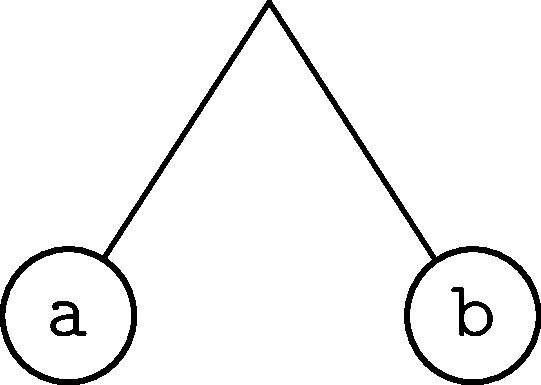
\includegraphics[width=0.135\textwidth]{lists-as-trees-1.pdf}}
  \hspace{0.1\textwidth}
  \subfigure[\texttt{(a b c)}]{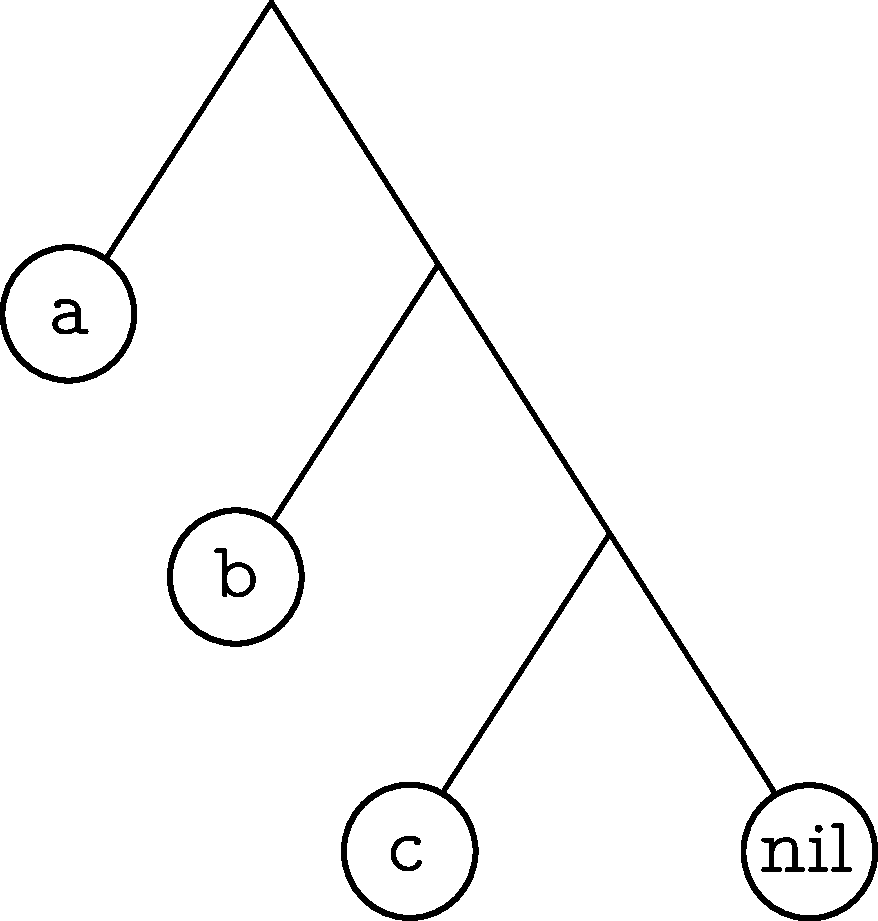
\includegraphics[width=0.21\textwidth]{lists-as-trees-2.pdf}}
  \hspace{0.1\textwidth}
  \subfigure[\texttt{(a b (c d))}]{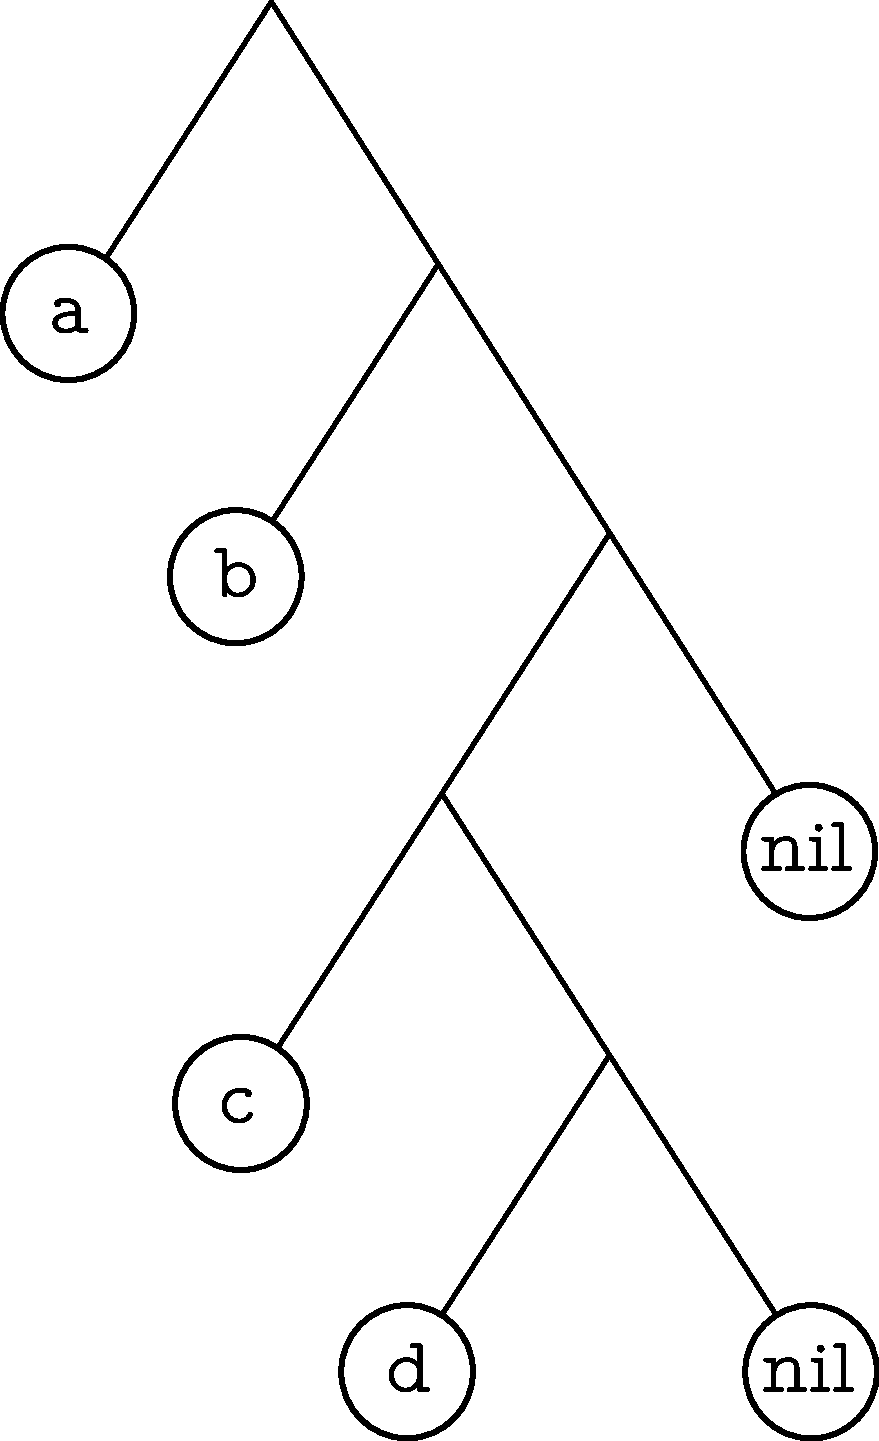
\includegraphics[width=0.21\textwidth]{lists-as-trees-3.pdf}}
  \caption{用列表表示的树}
  \label{fig:lists_as_trees}
\end{figure}

Lisp 的列表是一种全能型的数据结构\index{lists!uses for}。举例来说,列表能表示序列,集合,映射,数组,
以及树\index{trees 树}。目前有几种不同的方法来用列表表示树。
最常用的一种是把列表看作二叉树\index{lists!as binary trees},二叉树的左子树是~car,右子树则是~cdr。
(实际上,这往往就是列表的内部实现。) 图~\ref{fig:lists_as_trees}
中有三个例子,分别展示了列表以及它们所表示的树。其中,树上的每个内部节点
都对应着相应列表\index{dotted list}的\cons{}表示中的一个点,因而把列表看成下面的形式能更容易
理解这种的树型结构:
\begin{lstlisting}
    (a b c)     = (a . (b . (c . nil)))
    (a b (c d)) = (a . (b . ((c . (d . nil)) . nil)))
\end{lstlisting}
任意列表都可以看成一颗二叉树。同样的,Common Lisp 里也有其它一些成对的函数,它们之间的区别与~\texttt{copy-list}\index{copy-list@\texttt{copy-list}} 
和~\texttt{copy-tree}\index{copy-tree@\texttt{copy-tree}} 两者的区别类似。
前者把列表当作一个序列来处理,即如果碰到列表中含有子列表的情况,
那么子列表作为序列里的元素,是不会被复制的:
\begin{lstlisting}
> (setq x     '(a b)
        listx (list x 1))
((A B) 1)
> (eq x (car (copy-list listx)))
T
\end{lstlisting}
与之相对,\texttt{copy-tree} 会把列表当成树来拷贝,即把子列表视为子树,
所以子列表也一样会被复制:
\begin{lstlisting}
> (eq x (car (copy-tree listx)))
NIL
\end{lstlisting}
我们可以自己定义一个~\texttt{copy-tree},见下面的代码:
\begin{lstlisting}
(defun our-copy-tree (tree)
  (if (atom tree)
      tree
      (cons (our-copy-tree (car tree))
            (if (cdr tree) (our-copy-tree (cdr tree))))))
\end{lstlisting}
可以看出,上面的定义是一种常用模式的特例。(接下来,有些函数的写法会稍显
不自然,这是为了让这个模式变得更明显一些。) 不妨看看下面的例子,它能够
统计出一棵树里叶子节点\index{trees 树!leaves of 叶子}的数量:
\begin{lstlisting}
(defun count-leaves (tree)
  (if (atom tree)
      1
      (1+ (count-leaves (car tree))
          (or (if (cdr tree) (count-leaves (cdr tree)))
              1))))
\end{lstlisting}
一棵树上的叶子数会多于当它被表示成列表的形式时列表中原子的数量。
\begin{lstlisting}
> (count-leaves '((a b (c d)) (e) f))
10
\end{lstlisting}
而树用~\emph{\cons{}} 的形式来表示时,你可以注意到树上每个叶子都对应一个原子。
在\cons{}表示中,\texttt{((a b (c d)) (e) f)} 中有四个~\texttt{nil} 是在
列表表示中看不到的~(每对括弧都有一个),所以~\texttt{count-leaves} 的返回值是~10。

在上一章中,我们定义了几个用来操作树的\utility{}。比如说,\texttt{flatten}\index{flatten@\texttt{flatten}} 
(第~\pageref{fig:doubly-recursive_list_utilities} 页) 接受一颗树,
并返回一个含有树上所有原子的列表。换句话说,如果你传给~\texttt{flatten} 一个
嵌套列表,你所得到的返回列表和前面的列表形式相同,不过除了最外面那对之外,
其它的括弧都不见了:
\begin{lstlisting}
> (flatten '((a b (c d)) (e) f ()))
(A B C D E F)
\end{lstlisting}
这个函数也可以像下面那样定义~(尽管效率有点低):
\begin{lstlisting}
(defun flatten (tree)
  (if (atom tree)
      (mklist tree)
      (nconc (flatten (car tree))
             (if (cdr tree) (flatten (cdr tree))))))
\end{lstlisting}

最后,看一下~\texttt{rfind-if}\index{rfind-if@\texttt{rfind-if}},它是~\texttt{find-if}\index{find-if@\texttt{find-if}!version for trees} 的递归版本。
\texttt{rfind-if} 不仅能用在线性的列表上,而且对树也一样适用:
\begin{lstlisting}
(defun rfind-if (fn tree)
  (if (atom tree)
      (and (funcall fn tree) tree)
      (or (rfind-if fn (car tree))
          (if (cdr tree) (rfind-if fn (cdr tree))))))
\end{lstlisting}
为了让~\texttt{find-if} 的应用范围更广,使之能用于树结构,必须
在两者中择一: 让它仅仅搜索叶子节点,或是搜索整个子树。
我们的~\texttt{rfind-if}\note{73} 选择了前者,因而调用方就可以认为:
作为第一个参数传入的函数只会用在原子上:
\begin{lstlisting}
> (rfind-if (fint #'numberp #'oddp) '(2 (3 4) 5))
3
\end{lstlisting}

\texttt{copy-tree},\texttt{count-leaves},\texttt{flatten} 和~
\texttt{rfind-if},这四个函数的形式竟然如此相似。实际上,它们都是
某个原型函数的特例,这个原型函数被用来进行子树上的递归操作。和之前
对待~cdr 上递归的态度一样,我们不希望让这个原型默默无闻地埋没在代码当中,
相反,我们要写一个函数来产生这种原型函数的实例。

要得到原型本身,让我们先研究一下这些函数,找出哪些部分是不属于模式的。
从根本上来说,\texttt{our-copy-tree} 有两种情形:
\begin{enumerate}
\item 基本的情况下,函数直接把参数作为返回值返回
\item 在递归的时候,函数对左子树~(car) 的递归结果和右子树~(cdr) 
      的递归结果使用~\texttt{cons}
\end{enumerate}
因此,我们肯定可以通过调用一个有两个参数的构造函数,来表示~\texttt{our-copy-tree}:
\begin{lstlisting}
(ttrav #'cons #'identity)
\end{lstlisting}

图~\ref{fig:function_for_recursion_on_trees:ttrav} 中为~\texttt{ttrav} (``tree traverser'') 
的一种实现。在递归的情况下,我们传入的不是一个值,而是两个,一个对应左子树,
一个对应右子树。如果~\verb|base| 参数是个函数,那么将把当前叶子节点作为参数传给它。
在对线性列表进行递归操作时,基本情况的返回值总是~\verb|nil|,
不过在树结构的递归操作中,基本情况的值有可能是个更有意思的值,而且我们也许会需要用到它。

在~\verb|ttrav| 的帮助下,我们可以重新定义除~\verb|rfind-if| 之外前面提到的所有函数。
(这些函数在图~\ref{fig:functions_expressed_with_ttrav} 中可以找到。)
要定义~\verb|rfind-if|,需要更通用的树结构递归操作函数的生成器,
这种函数生成器能让我们控制递归调用发生的时机,以及是否继续递归。我们把一个函数作为传给~\verb|ttrav| 
的第一个参数,这个函数的参数将是递归调用的\emph{返回值}。对于通常的情形,
我们会改用另一个函数,让它接受两个闭包,闭包分别自行表示调用操作。这样,
就可以编写那些能自主控制递归过程的递归函数了。

\begin{figure}
\begin{lstlisting}
(defun ttrav (rec &optional (base #'identity))
  (labels ((self (tree)
                 (if (atom tree)
                     (if (functionp base)
                         (funcall base tree)
                         base)
                     (funcall rec (self (car tree))
                                  (if (cdr tree)
                                      (self (cdr tree)))))))
    #'self))
\end{lstlisting}
\caption{\label{fig:function_for_recursion_on_trees:ttrav}为在树上进行递归操作而设计的函数}
\index{ttrav@\texttt{ttrav}}
\end{figure}

\begin{figure}
\begin{lstlisting}
; our-copy-tree
(ttrav #'cons)

; count-leaves
(ttrav #'(lambda (l r) (+ l (or r 1))) 1)

; flatten
(ttrav #'nconc #'mklist)
\end{lstlisting}
\caption{\label{fig:functions_expressed_with_ttrav}用~\texttt{ttrav} 表示的函数}
\end{figure}

\begin{figure}
\begin{lstlisting}
(defun trec (rec &optional (base #'identiy))
  (labels
      ((self (tree)
             (if (atom tree)
                 (if (functionp base)
                     (funcall base tree)
                     base)
                 (funcall rec tree
                              #'(lambda ()
                                  (self (car tree)))
                              #'(lambda ()
                                  (if (cdr tree)
                                      (self (cdr tree))))))))
    #'self))
\end{lstlisting}
  \caption{\label{fig:function_for_recursion_on_trees:trec}为在树上进行递归操作而设计的函数}
  \index{trec@\texttt{trec}}
\end{figure}

用~\texttt{ttrav} 实现的函数通常会遍历整颗树。这样做对于像
~\texttt{count-leaves} 或者~\texttt{flatten} 这样的函数是没有问题的,
它们不管如何都会遍历全树。然而,我们需要~\texttt{rfind-if} 一发现
它所要找的元素就停止遍历。这个函数必须交给更通用的~\texttt{trec} 来生成,
见图~\ref{fig:function_for_recursion_on_trees:trec}。
\verb|trec| 的第二个参数应当是一个具有三个参数的函数,三个参数分别是:
当前的对象,以及两个递归调用。后两个参数将是用来表示对左子树和右子树进行
递归的两个闭包。使用~\verb|trec| 我们可以这样定义~\verb|flatten|:
\begin{lstlisting}
(trec #'(lambda (o l r) (nconc (funcall l) (funcall r)))
\end{lstlisting}
现在,我们同样可以把~\verb|rfind-if| 写成这样~(下面的例子用了~\verb|oddp|):
\begin{lstlisting}
(trec #'(lambda (o l r) (or (funcall l) (funcall r)))
      #'(lambda (tree) (and (oddp tree) tree)))
\end{lstlisting}

\section{何时构造函数}
\label{sec:when_to_build_functions}

很不幸,如果用构造函数,而非~sharp-quoted 的~lambda 表达式来表示
函数会在运行时让程序做一些不必要的工作。虽然~sharp-quoted 的~\lexpr
是一个常量,但是对构造函数的调用将会在运行时求值。如果你真的必须在运行
时执行这个调用,可能使用构造函数并非上策。不过,至少有的时候我们可以在事前就
调用这个构造函数。通过使用~\verb|#.|\index{\#.@\texttt{\#.}},即
~sharp-dot 读取宏,我们可以让
函数在读取期~(read-time) 就被构造出来。假设~\verb|compose| 和它的参数
在下面的表达式被读取时已经被定义了,那么我们可以这样写,举例如下:
\begin{lstlisting}
(find-if #.(compose #'oddp #'truncate) lst)
\end{lstlisting}
这样做的话,reader 就会对~\verb|compose| 的调用进行求值,求值得到的函
数则被作为常量安插在我们的代码之中。由于~\verb|oddp| 和~\verb|truncate| 
两者都是内置函数,所以在读取时对~\verb|compose| 进行估值可以被认为是
安全可行的,当然,前提是那个时候~\verb|compose| 自己已经加载了。

一般而言,由宏来完成函数复合或者合并,既简单容易,又提高了程序的性能。
这一点对函数拥有具有单独名字空间的~Common Lisp 来说尤其如此。
在介绍了宏的相关知识后,我们会在第~\ref{chap:macro_returning_functions} 章
故地重游,再次回到这一章中曾走到过的大多数山山水水,所不同的是,到那时
候你会骑上更纯种的宝马,配上更奢华的鞍具。

%%% Local Variables:
%%% coding: utf-8
%%% mode: latex
%%% TeX-master: "onlisp-cn"
%%% End:
